\documentclass[12pt,a4paper]{scrartcl}
\usepackage{geometry}
\usepackage{fancyhdr}
\usepackage{url}
\usepackage{csquotes}
\usepackage{amsmath}
\usepackage{amsthm}
\usepackage{amssymb}
\usepackage{graphicx}
\usepackage{subfigure}
\date{April 20, 2016}
\pagestyle{fancy}
\cfoot{\thepage}
\title{Interim report}
\subtitle{Distributed financial data forecaster}
\author{Wang Youan\\{\small Supervised by: YIP Chi Lap}}
\geometry{left=2cm, right=2cm, top=2cm, bottom=2cm}
\bibliographystyle{abbrv}
\graphicspath{{images/}}
\setlength{\parindent}{15pt}
\begin{document}
	\maketitle
	\section{Introduction}
	It is human beings' common goal to make life easier and more comfortable. Wealth can bring help to achieve this goal. That's why there are so many works done to predict the stock price. As stock market is a very complex (non-linear) and volatile system with many factors (such as companies' performance, domestic economies, festivals, seasons, etc.)\cite{chen1986economic}, it is difficult to precisely predicted its daily behaviors. Besides, those factors usually have relationship with each other, and they will keep changing all the time. Hence, investors and fund manager must maintain real-time monitoring of market behavior, so as to make the right trading decision.\\
	\indent With the development of machine learning and cloud computing technologies, people find a new way to analyze many factors of stock price at a time without too much manual cost. There are many works towards prediction have been attempted, includes neural network\cite{kimoto1990stock,naeini2010stock}, multi-class support vector machine\cite{kercheval2015modelling}, linear and polynomial regression\cite{nunnostock,alexanderstock}, random forest\cite{alexanderstock,lauretto2013evaluation}. However, none of those models have become widely accepted. 
	\section{Objectives}
	In this study, I will try to challenge the problem of real time prediction. The outcome of this dissertation is a distributed prediction system running on Apache Spark\cite{apache_spark} combining machine learning technique and technical, fundamental analysis together to predict stock price and trends.
	\section{Current Methods}
	From "Efficient Market Hypothesis"\cite{basu1977investment,sewell2011history,vacha2005dynamical}, we can find that the changes of stock price follows a random walk which could be explained via Brownian motion techniques. I've tried  the below methods to simulate such motion and to make a prediction.
	\subsection{Stochastic gradient descent}
	\textbf{Stochastic Gradient Descent (SGD)} is a simple but efficient approach to solve supervised learning problem on large scale\cite{bottou2010large}, which makes it very suitable to be used for long term price prediction. The model of loss in my model is \cite{spark_documentation},
	\begin{equation}
		\label{eq:SGD}
		L(w;x,y):=\frac{1}{2}(w^Tx-y)^2
	\end{equation}
	Where L is loss, $ x $ is the input vector and $ w $ is the weight vector.
	\subsection{Random Forest}
	Random Forest is a special type of decision trees and was first introduced by Leo Breiman \cite{breiman2001random}. This algorithm constructs a multitude of decision trees at training time and outputs the mean prediction of those individual trees. This methods is designed to eliminate the overfitting of decision trees.
	\subsection{Apache Spark}
	Apache Spark, which is first developed at the UC Berkeley AMPLab and has been contributed to the Apache Software Foundation, is a fast and general engine for large-scale data processing\cite{ryza2015advanced}. Spark inherits MapReduce's linear scalability and fault tolerance, and extends it in three ways,
	\begin{itemize}
		\item First, instead relying on a map-then-reduce format, Spark executes operators using directed acyclic graph (DAG), which means that while MapReduce must write intermediate results to the file system, Spark can transmit them directly to the next step. This makes Spark much faster.
		\item Second, highly accessible. Spark offers simple APIs in Python, Java, Scala, SQL and R. Besides, users can use it interactively from the Scala, Python and R shells. Those features make Spark more easy to use.
		\item Third, Spark integrates closely with other Big Data tools. For example, \enquote{Spark can run on Hadoop, Mesos, standalone, or in the cloud. It can access diverse data sources including HDFS, Cassandra, HBase, and S3}\cite{apache_spark}.
	\end{itemize}
	\section{Works has been done}
	Before the end of April 2016, I've finish the below works,
	\subsection{Distributed System Deploy and Learning}
	I use 3 virtual machines, each have 2G RAM and a vcore, details can be find in figure~\ref{fig:environment}
	\begin{figure}[ht]
		\centering
		\subfigure[Virtual Machines]{
			\centering
			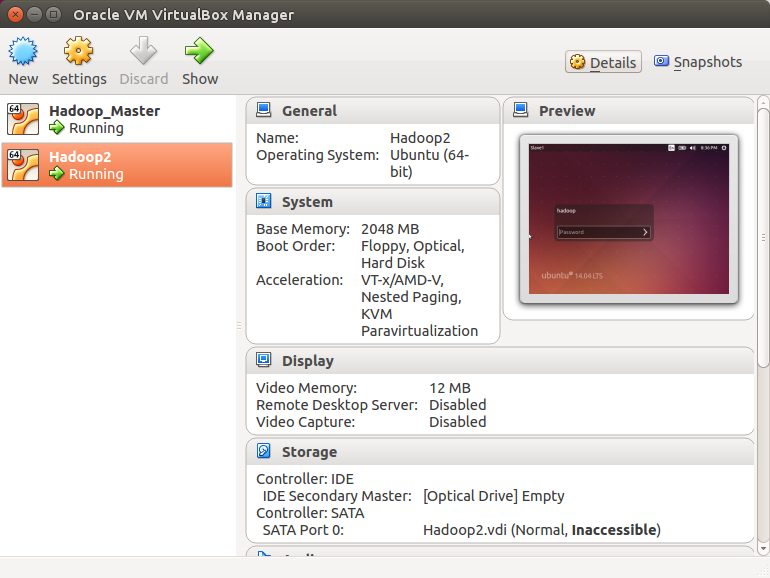
\includegraphics[width=.4\linewidth]{environments}
			\label{fig:vm}
		}
		\subfigure[Spark Web UI]{
			\centering
			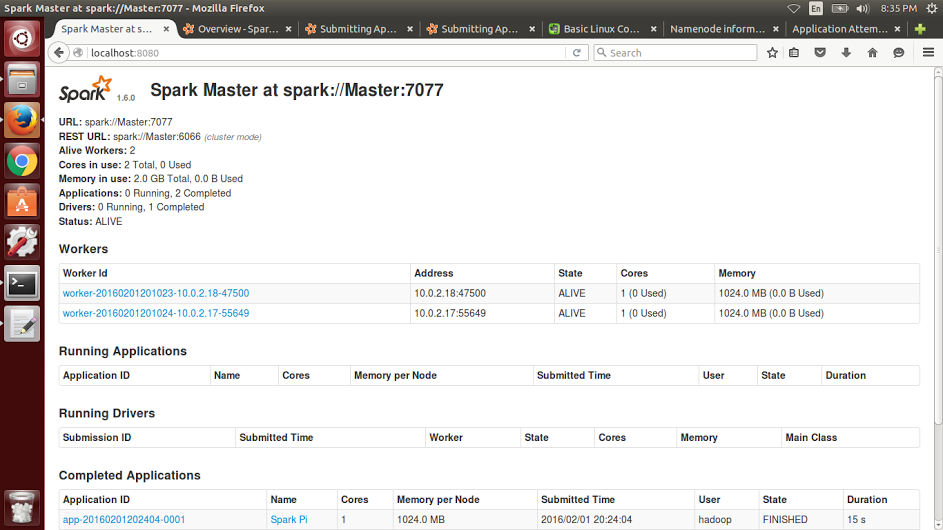
\includegraphics[width=.4\linewidth]{spark_deploy}
			\label{fig:spark}
		}
		\caption{Environment of my Cluster}
		\label{fig:environment}
	\end{figure} 
	Besides, the deployment, I can also make use of the distributed system to build simple predict model, and analyze stock data.
	\subsection{Financial Data Collect and Preliminary model}
	The daily stock data is collected from Yahoo Finance!. For further extension (use artificial neural network\cite{nayak2014impact}), the trained price will be first normalized based on the equation~\ref{eq:normalize}.
	\begin{equation}
		\label{eq:normalize}
		price = \frac{2\times price - (Max_{price}+Min_{Price})}{Max_Price-Min_Price}
	\end{equation}
	In this study, I choose mean absolute deviation(MAD, equation~\ref{eq:MAD}), mean absolute percentage error(MAPE, equation~\ref{eq:MAPE}) and mean squared error (MSE, equation~\ref{eq:MSE}) as prediction criteria.
	Compare of Normalize and Non-Normalize can be found in figure~\ref{fig:non_vs_nor} and figure~\ref{fig:mse_mad}. I use Linear Regression with SGD model, and the input values are 5 days average close and open price, highest and lowest price during the five days. 
	\begin{figure}[ht]
		\centering
		\subfigure[Prediction of HK \& CHINA GAS (0003.HK)]{
			\centering
			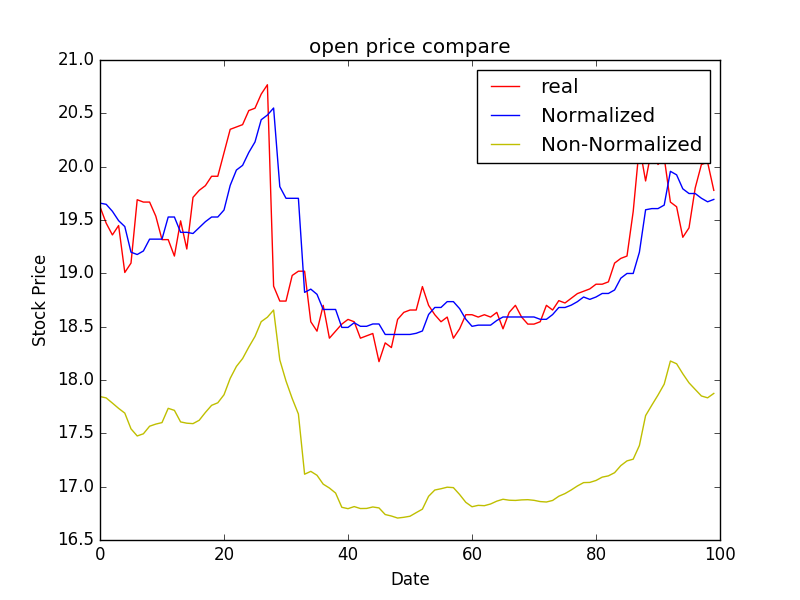
\includegraphics[width=.4\linewidth]{0003_HK}
			\label{fig:Non_Normalize}
		}
		\subfigure[Prediction of CLP HOLDINGS (0002.HK)]{
			\centering
			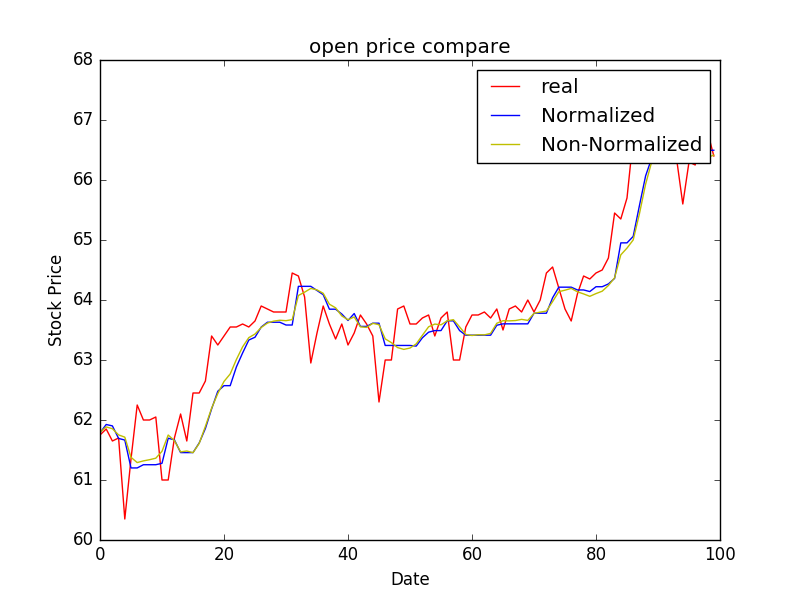
\includegraphics[width=.4\linewidth]{0002_HK}
			\label{fig:Normalize_Better}
		}
		\caption{Compare between Normalized and Non-Normalized data}
		\label{fig:non_vs_nor}
	\end{figure}
	\begin{figure}[ht]
		\centering
		\subfigure[MSE Compare]{
			\centering
			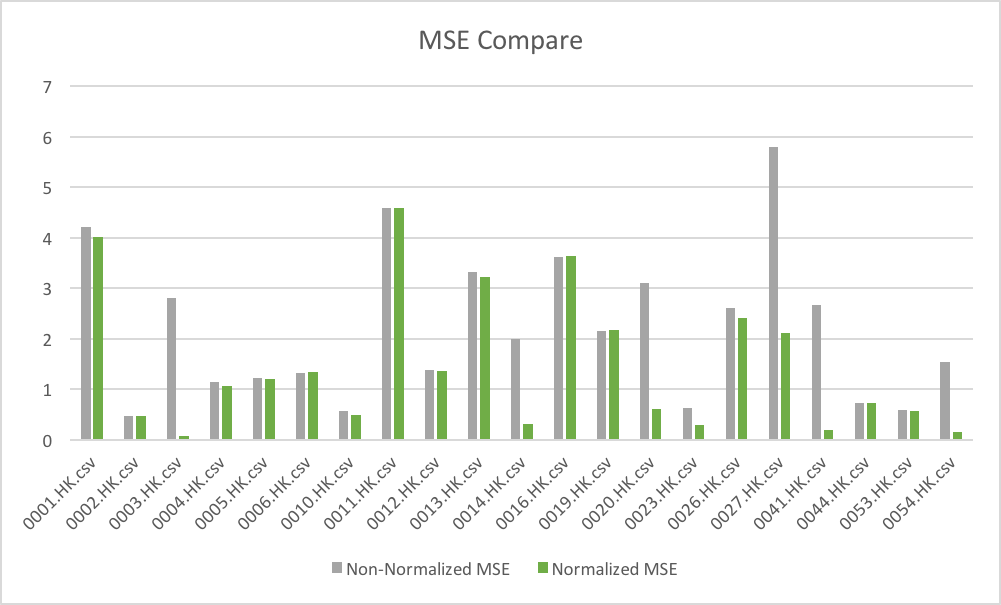
\includegraphics[width=.4\linewidth]{MSE}
			\label{fig:MSE}
		}
		\subfigure[MAD compare]{
			\centering
			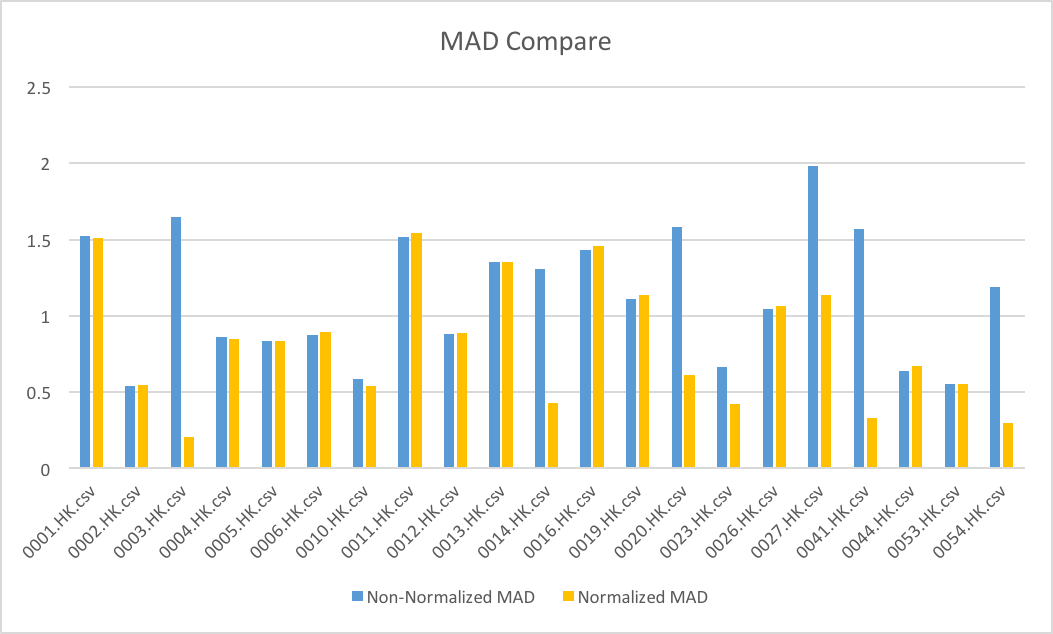
\includegraphics[width=.4\linewidth]{MAD}
			\label{fig:MAD}
		}
		\subfigure[MAPE compare]{
			\centering
			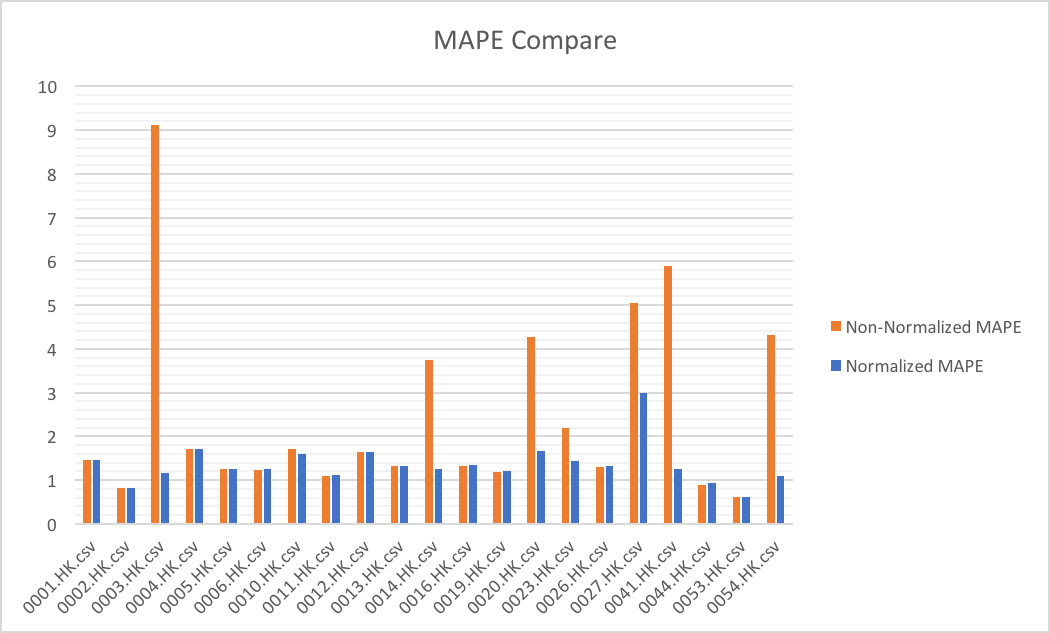
\includegraphics[width=.4\linewidth]{MAPE}
			\label{fig:MAPE}
		}
		\caption{Compare between Normalized and Non-Normalized data 2}
		\label{fig:mse_mad}
	\end{figure}
	\begin{gather}
	\label{eq:MAD}
	MAD = \frac{1}{|ValidationSet|}\sum|price_{forecast}-price_{real}|\\
	\label{eq:MAPE}
	MAPE = \frac{1}{|ValidationSet|}\sum|\frac{price_{forecast}-price_{real}}{price_{real}}|\\
	\label{eq:MSE}
	MSE = \frac{1}{|ValidationSet|}\sum(price_{forecast}-price_{real})^2
	\end{gather}
	From above results we can find that Normalized data is more reliable than Non-normalized prediction.
	\subsection{Dissertation Webpage}
	Thanks to \cite{1_miller_2016}, where I download the template from. Current version so Dissertation Website as figure~\ref{fig:webpage} The URL of my web page is \url{http://i.cs.hku.hk/~msd15090/index.html}
	\begin{figure}[th]
		\centering
		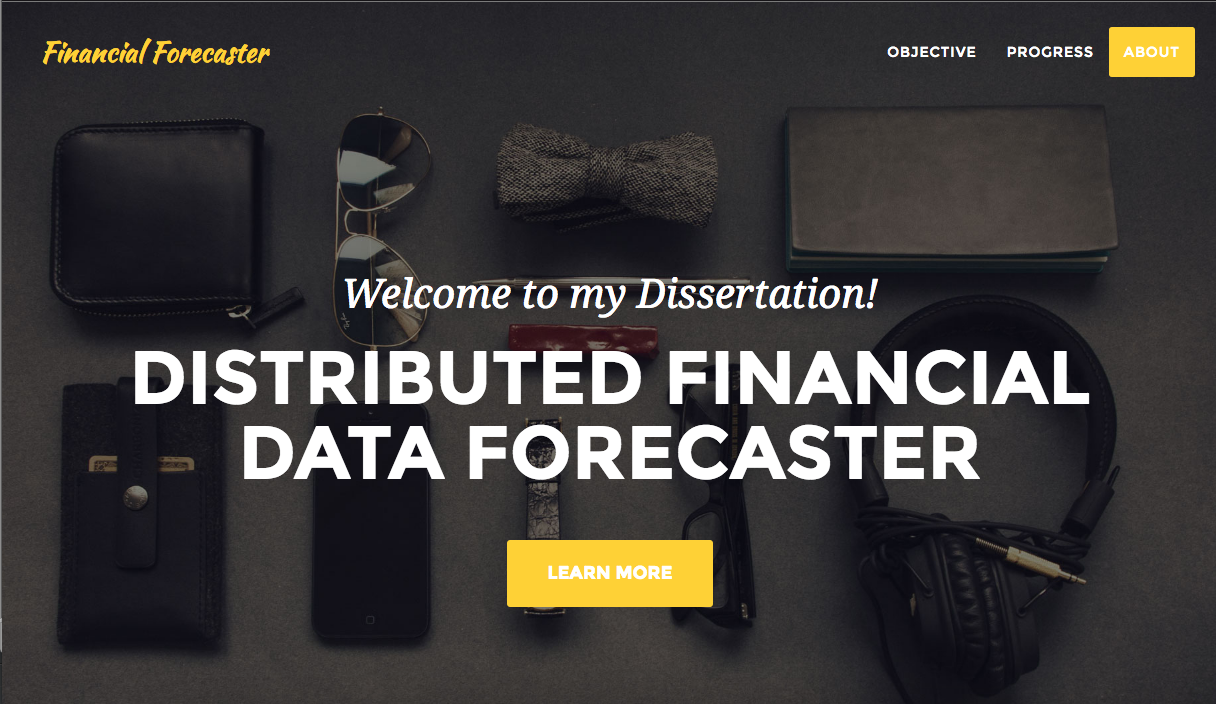
\includegraphics[width=0.6\linewidth]{webpage}
		\caption{Homepage of my dissertation web page}
		\label{fig:webpage}
	\end{figure}
	\section{Future Works}
	Based on the above works, my next works will includes,
	\begin{itemize}
		\item Build and tune an artificial neural network (ANN) based model to predict stock price. The idea of Neural Network is inspired by humans' nervous systems. Compare to traditional machine learning methods, e.g. linear regression and random forest, which are model based, ANN is self-adjusting methods based on training data\cite{kimoto1990stock}. This means that ANN has the ability of recognizing new patterns that it never learned before. I'll try to build an ANN model with the ability of self-adaptability.
		\item Add technical indicators and sentimental analysis. Only last n days price is not enough to reflect all the stock price features. Add some technical indicators, sentimental analysis and more features about date will help to improve the accuracy of my prediction model.
		\item Extends to intraday predict. My current research mainly focus on daily stock price. Intraday trading has much higher volatility than interday's, which makes it more profitable. After finishing the above two jobs, if time permits, I will try to use my model to predict hourly stock price.
	\end{itemize}
	Because of busy with other course, I may only finish 40\% of my total dissertation work. As all the other courses will come to end in the next month, I'll have enough time to finish the remaining dissertation works. 
	\bibliography{Interim_report}
\end{document}